\documentclass[11pt]{article}

\usepackage[margin=1in]{geometry}
\usepackage[T1]{fontenc}
\usepackage[utf8]{inputenc}
\usepackage{amsmath}
\usepackage{amssymb}
\usepackage{array}
\usepackage{booktabs}
\usepackage{enumitem}
\usepackage{graphicx}
\usepackage{longtable}
\usepackage[expansion=false]{microtype}
\usepackage{tikz}
\usetikzlibrary{arrows.meta,positioning}
\usepackage{hyperref}
\usepackage[numbers,sort&compress]{natbib}
\emergencystretch=2em

\hypersetup{
  colorlinks=true,
  linkcolor=blue,
  citecolor=blue,
  urlcolor=blue
}

\newcommand{\E}{\mathbb{E}}
\newcommand{\NPV}{\mathrm{NPV}}
\newcommand{\1}{\mathbf{1}}

\title{Estimating the Net Present Value of a New Credit Card Customer:\\
A Literature Survey and Modeling Framework for Retail Banks}
\author{Chak Wong}
\date{June 27, 2026}

\begin{document}
\maketitle

\begin{abstract}
Retail banks use credit card campaigns to acquire new customers, deepen existing
relationships, and shift payment activity onto proprietary products. The
commercial objective is not simply response, approval, activation, or first
purchase. It is incremental risk-adjusted net present value (NPV), net of
campaign cost, rewards, servicing, funding, capital, fraud, expected credit
loss, and cannibalization of the bank's existing products. This survey reviews
the literatures most relevant to that decision problem. Household-finance and
credit-card studies show that spending and borrowing are state dependent:
employment, income shocks, liquidity, credit limits, interest rates, policy
transfers, and macro shocks all alter card economics. Payment-choice and rewards
studies show that adoption and use are distinct outcomes, so a newly issued
card may remain inactive, cannibalize existing spend, or capture incremental
wallet share. Customer lifetime value and duration models provide useful
baselines for forecasting transaction frequency, monetary value, active status,
and relationship duration, but they must be integrated with credit risk and
balance-sheet economics for card portfolios. The paper proposes a modular
modeling architecture for estimating incremental credit-card NPV and identifies
where public literature is informative and where issuer-specific randomized or
quasi-experimental evidence is essential.
\end{abstract}

\section{Introduction}

A large U.S. retail bank considering a credit card campaign faces two related
business cases. First, the bank may market a card to a prospect who is not yet a
card customer. Second, it may offer a new card to an existing client, including
an existing bank customer with deposits or loans, or an existing cardholder who
could add another card. In both cases, the operational decision is often framed
as a propensity problem: who will respond, who will be approved, who will
activate, and who will spend. That framing is useful for funnel management, but
it is incomplete for capital allocation. The economically relevant object is a
profit or value objective, not a response score alone. This is consistent with
the direct-marketing literature on optimal selection, which ranks customers by
expected net return rather than by response probability alone
\citep{bult1995directmail}, and with the customer lifetime value (CLV) and
customer-equity literatures, which define customer value as a discounted stream
of expected future contribution \citep{berger1998clv,rust2004return,venkatesan2004clv}.
The credit-card setting adds bank-specific components---losses, capital,
funding, fraud, rewards, and cannibalization---to this familiar marketing
objective.

Let $i$ index customers, $t$ monthly time, and $a \in \mathcal{A}$ a marketing
or product action, such as a direct-mail offer, digital preapproval, branch
offer, balance-transfer campaign, rewards bonus, or product upgrade. In the
direct-mail formulation, the bank would mail customer $i$ when expected margin
times response probability exceeds contact cost:
\begin{equation}
  d_i^*
  =
  \1\{p_i m_i - c_i > 0\},
  \label{eq:direct-mail-profit}
\end{equation}
where $p_i$ is response probability, $m_i$ is conditional gross margin, and
$c_i$ is contact cost. In a CLV formulation, customer value is instead a
discounted contribution stream:
\begin{equation}
  \mathrm{CLV}_i
  =
  \E\left[
    \sum_{t=0}^{T} \delta_t \{R_{it}-C_{it}\}
    \,\middle|\, \mathcal{I}_{i0}
  \right].
  \label{eq:generic-clv}
\end{equation}
The card-acquisition problem combines these ideas with treatment effects:
\begin{equation}
  \Delta \NPV_i(a)
  =
  \E\left[
    \sum_{t=0}^{T}
      \delta_t
      \left\{
        \Delta R_{it}(a)
        - \Delta C_{it}(a)
        - \Delta L_{it}(a)
        - \Delta K_{it}(a)
      \right\}
    - A_i(a)
    \,\middle|\, \mathcal{I}_{i0}
  \right],
  \label{eq:incremental-npv}
\end{equation}
where $\Delta R_{it}$ is incremental revenue, $\Delta C_{it}$ is incremental
servicing, rewards, fraud, and funding cost, $\Delta L_{it}$ is expected credit
loss net of recovery, $\Delta K_{it}$ is capital or balance-sheet cost, $A_i(a)$
is acquisition and setup cost, and $\mathcal{I}_{i0}$ is information available at
the decision date. The increments are measured against the counterfactual in
which the customer does not receive action $a$.

Thus, Equation~\eqref{eq:incremental-npv} is not claimed to be a single
canonical equation from one credit-card paper. It is the synthesis needed for a
bank: Equation~\eqref{eq:direct-mail-profit} contributes the expected-profit
targeting logic, Equation~\eqref{eq:generic-clv} contributes the discounted
lifetime stream, and causal/uplift methods contribute the requirement that all
terms be incremental to the no-offer counterfactual.

This counterfactual is crucial. For an existing client, observed post-campaign
spend on a new card can be high even when incremental NPV is low: the card may
shift spend from the bank's old card, pull forward spend through a costly
promotion, or create balances whose losses exceed finance charges. Conversely, a
moderate activation probability can be valuable if it creates durable
incremental purchase volume, profitable revolving balances, and low servicing
and loss costs. The bank's literature problem is therefore not a search for a
single ``credit-card NPV paper.'' It is a synthesis problem across household
finance, payment choice, credit-card economics, causal marketing, and customer
lifetime value.

This paper is organized around three questions. Section~\ref{sec:macro}
reviews evidence on how market conditions, employment, income, and liquidity
alter spending and card economics. Section~\ref{sec:usage} reviews adoption,
activation, rewards, and use of new payment instruments. Section~\ref{sec:ltv}
reviews customer lifetime value and duration models for lifetime expenditure.
Section~\ref{sec:architecture} proposes a practical model architecture for a
bank. Section~\ref{sec:component-decomposition} develops a component
decomposition into losses, balances, PPNR, and portfolio-management overlays.
Section~\ref{sec:decision-pitfalls} addresses measurement and decision
pitfalls that arise when NPV is used across the card funnel.
Section~\ref{sec:validation} discusses empirical design and validation.
Section~\ref{sec:audit} records the source-support limits of this first-pass
survey.

\section{Market Conditions, Employment, and Propensity to Spend}
\label{sec:macro}

\subsection{Income, unemployment, and liquidity}

The first component of credit-card NPV is the customer's capacity and propensity
to spend. The relevant empirical papers do not estimate the bank's
Equation~\eqref{eq:incremental-npv} directly. They estimate causal or
quasi-causal effects of income, employment, and liquidity variables on spending
or debt. Their contribution to our model is a set of state variables and
elasticities for the spend, balance, and risk modules.

\citet{ganong2019unemployment} use de-identified bank account data to study
spending around unemployment and the predictable income drop at unemployment
insurance exhaustion. A stylized event-study version of the object is
\begin{equation}
  y_{i\tau}
  =
  \alpha_i + \lambda_\tau
  + \sum_{k \neq -1} \beta_k \1\{\tau_i = k\}
  + \varepsilon_{i\tau},
  \label{eq:unemployment-event-study}
\end{equation}
where $y_{i\tau}$ is spending for household $i$ at event time $\tau$ relative to
an unemployment or benefit-exhaustion event, $\alpha_i$ absorbs household fixed
effects, and the $\beta_k$ trace the spending path around the event. The
important modeling implication is not merely ``unemployment matters.'' It is
that the card spend forecast should include event-time variables such as job
loss, payroll interruption, benefit receipt, and benefit exhaustion, because
spend can move non-smoothly around predictable income events.

\citet{johnson2004rebates} study the 2001 tax rebates using variation in rebate
timing. A stylized specification is
\begin{equation}
  \Delta c_{it}
  =
  \alpha_i + \lambda_t
  + \gamma\,\mathrm{Rebate}_{it}
  + \eta' H_i\,\mathrm{Rebate}_{it}
  + u_{it},
  \label{eq:rebate-mpc}
\end{equation}
where $\gamma$ is a marginal propensity to consume out of the transfer and
$H_i$ contains heterogeneity variables such as income or liquid-wealth status.
For a credit-card model, this says that transfers, payroll changes, and liquid
wealth proxies should enter monthly purchase-volume and payment-rate equations,
with heterogeneous effects. It does not identify the share of extra consumption
that will route through our card.

\citet{gross2001liquidity} provide the closest direct credit-card evidence.
They study account-level card and bureau data and estimate how debt responds to
credit limits and interest rates. A stylized account-level equation is
\begin{equation}
  \Delta B_{it}
  =
  \alpha_i + \lambda_t
  + \theta\,\Delta \mathrm{Limit}_{it}
  + \rho\,\Delta \mathrm{APR}_{it}
  + \psi' X_{it}
  + e_{it},
  \label{eq:limit-apr-response}
\end{equation}
with stronger responses among initially high-utilization or liquidity-constrained
borrowers. This should enter our future model through the balance and payment
modules: line assignment and APR are not passive controls; they are treatment
components that affect revolving balances, utilization, finance charges, and
expected loss.

\subsection{Rates, regulation, and product terms}

Credit-card NPV is also shaped by prices, fees, disclosures, repayment rules,
and regulatory constraints. \citet{agarwal2013cardact} study the Credit Card
Accountability Responsibility and Disclosure Act using a large account-level
card panel. The paper is not a spend-propensity model, and this survey should
not use it as if it supplied a universal activation or balance elasticity. Its
modeling value is different: it shows that product terms are governed economic
objects. Fees, disclosures, and repayment nudges can change both issuer revenue
components and consumer repayment behavior, so the NPV model cannot treat APRs,
fees, and promotional terms as free scalar revenue add-ons.

Formally, the campaign action should be represented as a vector of product
terms, not as a binary contact flag:
\begin{equation}
  a_{it}
  =
  \left(
    \ell_{it}, r^{\mathrm{purchase}}_{it},
    r^{\mathrm{cash}}_{it}, r^{\mathrm{BT}}_{it},
    r^{\mathrm{promo}}_{it}, T^{\mathrm{promo}}_{it},
    f_{it}, q_{it}, b_{it}, d_{it}
  \right)
  \in \mathcal{A}_{it}(X_{it},M_{gt},G_t).
  \label{eq:offer-vector}
\end{equation}
Here $\ell$ is the credit line; the $r$ terms are purchase, cash-advance,
balance-transfer, and promotional APRs; $T^{\mathrm{promo}}$ is promotional
duration; $f$ is the vector of annual, late, balance-transfer, cash-advance,
foreign-transaction, and waiver terms; $q$ is the reward earn or redemption
schedule; $b$ is a signup or statement-credit bonus; and $d$ is the disclosure,
minimum-payment, autopay, and digital-wallet provisioning design. The feasible
set $\mathcal{A}_{it}$ is indexed by customer state, macro state, and governance
state $G_t$ because underwriting policy, compliance rules, disclosure
requirements, risk appetite, pricing floors, and operational constraints limit
which offers can be made.

This notation connects the CARD Act evidence to the later NPV architecture in
two ways. First, regulation changes the feasible set and sometimes the cash-flow
mapping:
\begin{align}
  a_{it} &\in \mathcal{A}_{it}(G_t), \label{eq:regulated-action-set}\\
  CF_{i,t+1} &= c(Z_{it},X_{it},M_{gt},a_{it};G_t).
       \label{eq:regulated-cashflow-map}
\end{align}
A rule change, fee cap, disclosure change, or repayment-allocation rule is
therefore not merely an external dummy variable. It changes either the offers
available to the bank or the function that maps behavior into interest, fees,
payments, and balances. Second, product terms are treatments that enter the
behavioral transition system. A reduced-form version is
\begin{align}
  \Pr(Z_{i,t+1}=z'\mid Z_{it},X_{it},M_{gt},a_{it},G_t),
       \label{eq:terms-transition}\\
  \E[Y_{i,t+1}\mid Z_{i,t+1},X_{it},M_{gt},a_{it},G_t],
       \qquad
  Y\in\{S,B,Pay,D,Q\}.
       \label{eq:terms-outcomes}
\end{align}
Thus APR, line, fees, rewards, and disclosures can affect activation, purchase
volume, revolving balances, payments, delinquency, rewards liability, servicing
cost, and attrition. They should not be appended only after a response model has
already selected customers.

The mathematical bridge to \citet{gross2001liquidity} is direct. Equation
\eqref{eq:limit-apr-response} says that limit and APR changes can move card
debt, especially for liquidity-constrained accounts. In the NPV engine, the
same terms must feed both revenue and risk:
\begin{align}
  B_{i,t+1}
    &=
      g_B(B_{it},Pay_{it},S_{it},\ell_{it},r_{it},f_{it},
          X_{it},M_{gt}) + \varepsilon^B_{i,t+1},
      \label{eq:terms-balance}\\
  Int_{i,t+1}
    &=
      r^{\mathrm{revolve}}_{it}\,
      B^{\mathrm{revolve}}_{i,t+1}
      + r^{\mathrm{cash}}_{it}\,
      B^{\mathrm{cash}}_{i,t+1}
      + r^{\mathrm{BT}}_{it}\,
      B^{\mathrm{BT}}_{i,t+1},
      \label{eq:terms-interest}\\
  EL_{i,t+1}
    &=
      PD_{i,t+1}(Z_{it},U_{it},X_{it},M_{gt},a_{it})\,
      LGD_{i,t+1}\,
      EAD_{i,t+1}(B_{i,t+1},\ell_{it},a_{it}).
      \label{eq:terms-loss}
\end{align}
Raising APR can mechanically increase the rate applied to revolving balances,
but it can also change borrowing, payment, attrition, and default behavior.
Increasing the line can raise usage and finance revenue, but it can also raise
utilization dynamics, exposure at default, capital, and downside risk. The
correct object for decisioning is therefore a total derivative of value with
respect to the governed offer vector, not a partial revenue calculation holding
behavior fixed. Let
$\mu_Y(a)=\E[Y_i(a)\mid\mathcal{I}_{it}]$ for
$Y\in\{Z,S,B,Pay,D,Q\}$. For any feasible local perturbation $v$ of the offer
vector,
\begin{align}
  D_v\E[\Delta \NPV_i(a)]
  &=
  \left.
  \nabla_a \E[\Delta \NPV_i(a,\mu)]^\top v
  \right|_{\mu=\mu(a)}
  \nonumber\\
  &\quad
  +
  \sum_{Y\in\{Z,S,B,Pay,D,Q\}}
  \left.
  \frac{\partial \E[\Delta \NPV_i(a,\mu)]}{\partial \mu_Y}
  \right|_{\mu=\mu(a)}
  D_v\mu_Y(a).
  \label{eq:terms-total-derivative}
\end{align}
The first term is the mechanical cash-flow effect of the term sheet; the second
term is the behavioral response channel. The second term is precisely why the
rates and regulation literature belongs before the usage, CLV, loss, balance,
and PPNR sections.

This also clarifies how product terms should be validated. The promotion
criterion is not whether a high-APR or high-fee offer raises modeled revenue
conditional on the same balance path. It is whether the feasible offer
$a\in\mathcal{A}_{it}(G_t)$ increases counterfactual value after behavioral
response, regulation, cannibalization, expected loss, capital, funding, rewards,
and servicing:
\begin{align}
  \Delta \NPV_i(a;G_t)
  &=
  -\Delta A_i(a)
  +
  \sum_{h=0}^{H}\delta_h\,
  \E\!\left[
  \begin{aligned}
    &\Delta PPNR_{i,t+h}(a;G_t)
    - \Delta EL_{i,t+h}(a;G_t)
    - \Delta K_{i,t+h}(a;G_t)\\
    &\quad
    + \Delta RelValue_{i,t+h}(a)
    \mid \mathcal{I}_{it}
  \end{aligned}
  \right].
  \label{eq:terms-to-npv}
\end{align}
Equation~\eqref{eq:terms-to-npv} is the handoff to the component decomposition
in Section~\ref{sec:component-decomposition}: promotional APRs and
balance-transfer terms become promo states and balance subledgers; fees and
waivers become non-interest income; rewards become expense and liability;
APR/line choices affect balances, EAD, and capital; disclosure and repayment
design enter payment and attrition transitions; and all terms remain subject to
the feasible governed action set.

\subsection{Macro shocks and category substitution}

Market shocks can change not only the level of spending but also the composition
of card spending. \citet{baker2020epidemic} use transaction-level household
financial data to study consumption during the COVID-19 shock. Their evidence
documents large changes in spending levels and categories during the epidemic.
For card NPV, category shifts matter because merchant-category mix affects
interchange, rewards expense, fraud risk, dispute rates, and charge-off
correlation. A recession, health shock, inflation shock, or local labor-market
shock can lower discretionary purchase volume while increasing borrowing demand
and credit risk.

The practical lesson is that spend models should be time varying and
category-aware. A customer with high pre-campaign grocery and travel spend is
not equally valuable in every macro state. A useful reduced-form component is
\begin{equation}
  \log(1+S_{ij,t+1})
  =
  \mu_i + \lambda_t + \kappa_j
  + \beta_j' M_{gt}
  + \chi_j' X_{it}
  + \omega_j' (M_{gt}\times X_{it})
  + \epsilon_{ij,t+1},
  \label{eq:category-spend}
\end{equation}
where $S_{ij,t+1}$ is spend in merchant category $j$, $M_{gt}$ is a local or
national macro vector for geography $g$, and $X_{it}$ includes customer
liquidity, payroll, utilization, and relationship variables. Equation
\eqref{eq:category-spend} is not lifted from one paper; it is the model slot
suggested by the income, liquidity, and macro-shock evidence.

\begin{table}[t]
\centering
\caption{How Section~\ref{sec:macro} evidence should enter a bank model.}
\label{tab:macro-to-model}
\begin{tabular}{p{0.22\linewidth}p{0.31\linewidth}p{0.37\linewidth}}
\toprule
Literature & Mathematical object & Model use \\
\midrule
\citet{ganong2019unemployment}
  & Event-time spending path around unemployment and benefit exhaustion.
  & Add job-loss, payroll interruption, benefit receipt, and exhaustion
    indicators to spend, payment, attrition, and loss modules. \\
\citet{johnson2004rebates}
  & Marginal propensity to consume out of transfer timing, with heterogeneity.
  & Add income/transfer shocks and liquidity interactions to spend and payment
    equations; do not assume routing to our card. \\
\citet{gross2001liquidity}
  & Account-level response of card debt to credit limits and APR.
  & Treat line and APR as treatment components affecting balances, finance
    revenue, utilization, and loss. \\
\citet{agarwal2013cardact}
  & Regulation-induced changes in fees, disclosures, repayment behavior, and
    issuer revenue components.
  & Treat APRs, fees, rewards, disclosures, and repayment rules as governed
    terms $a_{it}\in\mathcal{A}_{it}(G_t)$ that feed transition, balance, loss,
    PPNR, and promo-state equations rather than unconstrained revenue levers. \\
\citet{baker2020epidemic}
  & Transaction-level response of spending levels and categories to a macro
    shock.
  & Forecast category-level spend and interchange/rewards/fraud mix under
    macro scenarios. \\
\bottomrule
\end{tabular}
\end{table}

\section{Will the Newly Issued Card Be Used?}
\label{sec:usage}

\subsection{Adoption is not usage}

The second requested problem is the probability that a customer who receives a
new card will use that card. The payment-choice literature warns against
collapsing this into a single response probability. \citet{koulayev2012payment}
estimate a structural model of adoption and use of payment instruments by U.S.
consumers. Their central relevance here is that possession of a payment
instrument and use of that instrument are distinct choices. A customer may open
a card, activate it, and still use another issuer's card, debit card, cash, ACH,
or a digital wallet at the point of sale.

Mathematically, the useful structure is a two-stage adoption/use problem. A
stylized version is:
\begin{align}
  A_{im}^*
    &= Z_i'\alpha_m + \nu_{im}, \qquad
       A_{im} = \1\{A_{im}^*>0\}, \label{eq:adoption-latent}\\
  U_{ijm}
    &= X_{ijm}'\beta_m + \phi_m A_{im} + \varepsilon_{ijm},
       \qquad
       m^*_{ij}=\arg\max_{m \in \mathcal{M}_i} U_{ijm}.
       \label{eq:use-utility}
\end{align}
Here $A_{im}$ denotes whether consumer $i$ has adopted payment instrument $m$,
$U_{ijm}$ is the utility of using instrument $m$ for transaction context $j$,
and $\mathcal{M}_i$ is the set of adopted instruments available to consumer
$i$. The exact specification in \citet{koulayev2012payment} is richer, but
Equations~\eqref{eq:adoption-latent}--\eqref{eq:use-utility} capture the
modeling lesson for us: ``has the card'' gates the choice set, while ``uses the
card'' is a conditional payment-choice decision. Our card model should therefore
estimate activation and usage conditional on the customer's competing payment
portfolio rather than treating issuance as usage.

For a credit-card campaign, the operational funnel should therefore separate:
\begin{enumerate}[label=\arabic*.]
  \item offer exposure and response;
  \item application and approval;
  \item card opening and physical or digital activation;
  \item first purchase;
  \item repeated purchase;
  \item share-of-wallet capture;
  \item durable active state, dormancy, closure, or charge-off.
\end{enumerate}
Each transition has different covariates and different economic meaning.
Approval is partly a risk and underwriting outcome. Activation is partly a
friction and onboarding outcome. First purchase is an early usage outcome.
Share-of-wallet is a competitive payment-routing outcome. Durable activity is a
lifetime-value outcome.

\subsection{Rewards, reactivation, and early spend}

Rewards can alter usage, but the bank must distinguish profitable use from
costly promotional pull-forward. \citet{agarwal2010rewards} study cash-back
rewards using administrative data from a large U.S. financial institution. The
important point for our later model is that the paper is not just a qualitative
statement that ``rewards matter.'' It suggests three account-level response
objects:
\begin{align}
  A_{it}^{\mathrm{react}}
    &= \1\{S_{i,t-3:t-1}=0,\; S_{it}\geq s_0\}, \label{eq:reward-reactivation}\\
  S_{it}
    &= \text{monthly purchase spend on the card}, \label{eq:reward-spend-outcome}\\
  B_{it}
    &= \text{monthly card debt or revolving balance}. \label{eq:reward-debt-outcome}
\end{align}
Here $A_{it}^{\mathrm{react}}$ is a reactivation indicator among accounts that
were inactive before the reward, $S_{it}$ is the usage outcome, and $B_{it}$ is
the balance outcome. These are exactly the three objects a bank needs for a new
card: did the account become active, how much spend did it generate, and did it
also create debt exposure?

A reduced-form implementation for a randomized or quasi-randomized reward offer
can be written as
\begin{equation}
  Y_{it}
  =
  \alpha_i + \lambda_t
  + \tau\,\mathrm{Reward}_{it}
  + \eta' X_{it}
  + \epsilon_{it},
  \label{eq:rewards-treatment}
\end{equation}
where $Y_{it}$ may be purchase spend, revolving debt, or an indicator for
reactivation among previously inactive cardholders. The estimand is
\begin{equation}
  \tau_Y
  =
  \E[Y_{it}(r=1)-Y_{it}(r=0)],
  \label{eq:reward-ate}
\end{equation}
with $r$ denoting the reward treatment. In a bank implementation this should be
estimated heterogeneously,
\begin{equation}
  \tau_Y(x,r)
  =
  \E[Y_i(r)-Y_i(0)\mid X_i=x],
  \label{eq:reward-cate}
\end{equation}
where $X_i$ includes prior inactivity, existing card holdings, pre-period
merchant mix, line utilization, relationship depth, channel, credit quality, and
macro state. Equation~\eqref{eq:reward-cate} is the bridge from
\citet{agarwal2010rewards} to the later model: it gives a segment-level reward
response surface rather than a single portfolio average.

The output of this block should feed the NPV simulator in four places:
\begin{align}
  \Pr(Z_{i,t+1}=\mathrm{active}\mid Z_{it},X_{it},a)
    &\leftarrow
      \text{activation/reactivation effect}, \label{eq:reward-feed-active}\\
  \E[S_{i,t+1}\mid Z_{i,t+1},X_{it},a]
    &\leftarrow
      \text{spend effect}, \label{eq:reward-feed-spend}\\
  \E[B_{i,t+1}\mid Z_{i,t+1},X_{it},a]
    &\leftarrow
      \text{debt/balance effect}, \label{eq:reward-feed-balance}\\
  C^{\mathrm{reward}}_{i,t+1}(a)
    &= q_a S_{i,t+1} + F_a + R^{\mathrm{signup}}_a,
      \label{eq:reward-cost}
\end{align}
where $q_a$ is the earn rate or reward cost per dollar, $F_a$ is fixed program
cost, and $R^{\mathrm{signup}}_a$ is signup or statement-credit cost. The
promotion is attractive only if the incremental contribution implied by
\eqref{eq:reward-feed-active}--\eqref{eq:reward-cost} is positive after
cannibalization and losses. This is the concrete way to avoid importing a
headline reward effect as if it were a universal activation parameter.

Behavioral evidence also suggests that payment instruments can affect purchase
behavior. \citet{prelec2001creditcard} find in experimental settings that
willingness to pay can be higher under credit-card payment than cash payment.
For a bank NPV model, this is mechanism evidence: payment method may change the
purchase decision, not simply route a fixed purchase through a different rail.
The result is not a portfolio-level NPV estimate and should not be used as a
direct calibration without issuer data.

The conservative model use is a mechanism prior for the ticket-size component.
Let $N_{ijt}$ be transaction count in category $j$ and $\bar{s}_{ijt}$ average
ticket size. Then
\begin{align}
  S_{ijt} &= N_{ijt}\bar{s}_{ijt}, \label{eq:spend-count-ticket}\\
  \log \bar{s}_{ij,t+1}
    &= \mu_i+\kappa_j+\beta'X_{it}
       +\theta_1 \mathrm{CreditCard}_{ij,t+1}
       +\theta_2 \mathrm{RewardSalience}_{ij,t+1}
       +\epsilon_{ij,t+1}.
       \label{eq:ticket-size-payment}
\end{align}
The \citet{prelec2001creditcard} result supports allowing
$\theta_1$ or $\theta_2$ to differ from zero, but the bank must estimate those
parameters with transaction data. This block is explanatory unless validated on
issuer data; it should not be a hard-coded multiplier in NPV.

\subsection{Cannibalization and incremental usage}

For existing clients, the central challenge is cannibalization. A newly issued
card can create genuinely incremental spend, shift spend from another issuer,
shift spend from the bank's existing card, move checking/debit activity onto
credit, or induce balances whose loss and reward costs exceed revenue. To make
this estimable, define the following observed spend aggregates over horizon
$H$:
\begin{align}
  S^{\mathrm{new}}_{iH}
    &= \text{spend on the newly issued card}, \\
  S^{\mathrm{oldbank}}_{iH}
    &= \text{spend on the bank's pre-existing cards}, \\
  S^{\mathrm{debit}}_{iH}
    &= \text{bank-observed debit/checking purchase activity}, \\
  S^{\mathrm{bank}}_{iH}
    &= S^{\mathrm{new}}_{iH}+S^{\mathrm{oldbank}}_{iH}.
\end{align}
When outside-card spend is not observed, competitor-card substitution is latent
and must be inferred from bureau/payment-network aggregates, wallet estimates,
or experimental lift in total bank spend. The estimands are:
\begin{align}
  \tau_i^{\mathrm{new\ card\ spend}}(a)
    &=
    \E[S^{\mathrm{new}}_{i,t:t+H}(a)
      - S^{\mathrm{new}}_{i,t:t+H}(0)\mid \mathcal{I}_{it}],
      \label{eq:new-card-lift}\\
  \tau_i^{\mathrm{bank\ spend}}(a)
    &=
    \E[S^{\mathrm{all\ bank\ cards}}_{i,t:t+H}(a)
      - S^{\mathrm{all\ bank\ cards}}_{i,t:t+H}(0)\mid \mathcal{I}_{it}],
      \label{eq:bank-spend-lift}\\
  \mathrm{Cannibalization}_i(a)
    &=
    \tau_i^{\mathrm{new\ card\ spend}}(a)
      - \tau_i^{\mathrm{bank\ spend}}(a).
      \label{eq:cannibalization}
\end{align}
Equation~\eqref{eq:new-card-lift} can be positive while
Equation~\eqref{eq:bank-spend-lift} is small or even negative. That is why
new-card activation and new-card spend are not sufficient promotion criteria.

In a randomized campaign, these are directly estimable by treatment-control
differences:
\begin{align}
  \widehat{\tau}^{\mathrm{new}}(x)
    &=
    \E[S^{\mathrm{new}}_{iH}\mid A_i=1,X_i=x]
    -\E[S^{\mathrm{new}}_{iH}\mid A_i=0,X_i=x],
    \label{eq:randomized-new}\\
  \widehat{\tau}^{\mathrm{bank}}(x)
    &=
    \E[S^{\mathrm{bank}}_{iH}\mid A_i=1,X_i=x]
    -\E[S^{\mathrm{bank}}_{iH}\mid A_i=0,X_i=x],
    \label{eq:randomized-bank}\\
  \widehat{\kappa}(x)
    &=
    1-\frac{\widehat{\tau}^{\mathrm{bank}}(x)}
            {\widehat{\tau}^{\mathrm{new}}(x)}
    \quad\text{when }\widehat{\tau}^{\mathrm{new}}(x)>0.
    \label{eq:cannibalization-rate}
\end{align}
Here $\widehat{\kappa}(x)$ is the estimated cannibalization rate from the bank's
own existing-card book. If $\widehat{\kappa}(x)$ is close to one, most new-card
spend is shifted from old bank cards; if it is close to zero, new-card spend is
mostly incremental to the bank. If it is negative, the new card may also lift old
bank card spend, for example through relationship deepening.

The latent competitor-transfer component can be represented as
\begin{equation}
  \tau_i^{\mathrm{competitor\ shift}}(a)
  =
  \tau_i^{\mathrm{bank\ spend}}(a)
  - \tau_i^{\mathrm{debit\ shift}}(a)
  - \tau_i^{\mathrm{new\ consumption}}(a),
  \label{eq:competitor-shift}
\end{equation}
The debit-shift term can sometimes be estimated from the bank's checking and
debit data. The new-consumption term is harder to identify without network or
merchant-panel data. Equation~\eqref{eq:competitor-shift} should therefore be
treated as a decomposition with an uncertainty interval, not as a precisely
observed quantity.

Randomized campaign holdouts are the cleanest way to separate organic
propensity from treatment effect. When randomization is unavailable, the
causal-inference and uplift literatures provide tools, but they do not remove
the need for credible identification. The propensity-score framework of
\citet{rosenbaum1983propensity}, true-lift marketing models such as
\citet{lo2002true}, causal forests \citep{wager2018causalforests}, and
double/debiased machine learning \citep{chernozhukov2018dml} are useful
methodological references. In a regulated bank environment, they should be used
with overlap checks, sensitivity analysis, segment calibration, and careful
model-governance review.

For later modeling, the cleanest operational implementation is to estimate a
conditional average treatment effect for each downstream outcome,
\begin{equation}
  \tau_Y(x)
  =
  \E[Y_i(1)-Y_i(0)\mid X_i=x],
  \label{eq:cate}
\end{equation}
where $Y$ may be activation, first purchase, first-90-day new-card spend,
all-bank-card spend, revolving balance, loss, or full NPV. The causal/uplift
module should feed the simulation engine by replacing raw predictions
$\E[Y_i\mid A_i=1,X_i]$ with counterfactual contrasts
$\E[Y_i(1)-Y_i(0)\mid X_i]$. If randomization is not available, the model must
record the identification assumption and cannot be promoted solely on predictive
fit.

The handoff to Equation~\eqref{eq:incremental-npv} is explicit. Let
$r_j^{\mathrm{int}}$ be net interchange by merchant category, $q_j(a)$ reward
cost by category and offer, $m^{\mathrm{finance}}_{it}$ net finance margin on
balances, and $\ell_{it}$ expected loss. Then a horizon-$H$ incremental
contribution block is
\begin{align}
  \Delta \Pi_{iH}(a)
    &=
    \sum_{j}
      \{r_j^{\mathrm{int}}-q_j(a)\}
      \widehat{\tau}^{\mathrm{bank}}_{ijH}(a)
    + \widehat{\tau}^{\mathrm{finance}}_{iH}(a)
    - \widehat{\tau}^{\mathrm{loss}}_{iH}(a)
    - C_i^{\mathrm{campaign}}(a)
    - C_i^{\mathrm{servicing}}(a),
    \label{eq:incremental-contribution}\\
  \Delta \NPV_i(a)
    &=
    \sum_{h=0}^{H}
      \delta_h\,\E[\Delta \Pi_{ih}(a)\mid \mathcal{I}_{i0}].
      \label{eq:cannibalization-to-npv}
\end{align}
The key design choice is that interchange and reward revenue use
$\widehat{\tau}^{\mathrm{bank}}$, not raw new-card spend
$S^{\mathrm{new}}$. This is how the cannibalization model changes the
optimization target.

\begin{table}[t]
\centering
\caption{How Section~\ref{sec:usage} evidence should enter a bank model.}
\label{tab:usage-to-model}
\begin{tabular}{p{0.22\linewidth}p{0.31\linewidth}p{0.37\linewidth}}
\toprule
Literature & Mathematical object & Model use \\
\midrule
\citet{koulayev2012payment}
  & Structural adoption and conditional use of payment instruments.
  & Separate opened/activated state from conditional card-use choice; include
    competing payment instruments and transaction context. \\
\citet{agarwal2010rewards}
  & Treatment effect of rewards on spend, debt, and reactivation.
  & Estimate $\tau_Y(x,r)$ for reactivation, spend, and balances; feed the
    activation transition, conditional spend, balance, and reward-cost blocks
    in Equations~\eqref{eq:reward-feed-active}--\eqref{eq:reward-cost}. \\
\citet{prelec2001creditcard}
  & Experimental effect of payment medium on willingness to pay.
  & Use as mechanism support for the ticket-size equation
    \eqref{eq:ticket-size-payment}; estimate the payment-medium coefficient on
    issuer transaction data before using it in NPV. \\
Uplift/CATE literature
  & $\E[Y(1)-Y(0)\mid X=x]$ for activation, spend, balance, loss, and NPV.
  & Estimate new-card lift, all-bank-card lift, and cannibalization in
    Equations~\eqref{eq:randomized-new}--\eqref{eq:cannibalization-rate}; feed
    incremental contribution through Equation~\eqref{eq:incremental-contribution}. \\
\bottomrule
\end{tabular}
\end{table}

\section{Lifetime Expenditure and Customer Lifetime Value}
\label{sec:ltv}

\subsection{Customer-base models}

The third requested problem is how to model lifetime expenditure of a credit
card user. Marketing science provides a natural starting point. \citet{schmittlein1987counting}
develop a model for inferring which customers are still active and what they
will do next from transaction timing and frequency. This is directly relevant
for card accounts because a customer can silently become inactive before formal
closure.

\citet{fader2005bgnbd} propose the BG/NBD model as a tractable alternative to
the Pareto/NBD model for predicting repeat-purchase behavior.
\citet{fader2005rfm} connect recency, frequency, and monetary value to customer
lifetime value. These models are useful baselines for transaction frequency,
active/dormant status, and spend per transaction. They are especially relevant
for transactors whose value is driven primarily by purchase volume and
interchange rather than finance charges.

Relationship duration is another core object. \citet{bolton1998duration} models
the duration of a customer's relationship with a continuous service provider.
Credit cards have similar duration dynamics: fees, service quality, fraud
events, line changes, disputes, rewards devaluations, and pricing changes can
alter retention, dormancy, and usage.

\subsection{Why card NPV is broader than plain CLV}

Credit cards are not a pure repeat-purchase setting. A bank needs the lifetime
path of at least six linked processes:
\begin{align}
  S_{it} &= \text{purchase spend and transaction count}, \\
  B_{it} &= \text{statement and revolving balance}, \\
  P_{it} &= \text{payment amount and payment rate}, \\
  D_{it} &= \text{delinquency/default state}, \\
  U_{it} &= \text{active, dormant, closed, or charged-off usage state}, \\
  Q_{it} &= \text{rewards, fraud, disputes, servicing, and other costs}.
\end{align}
These processes are jointly determined. High spend can be profitable when it is
durable and low loss, but low value when driven by high rewards cost or
low-margin categories. Revolving balances can raise interest income and
expected loss simultaneously. A durable active customer may be unprofitable if
servicing, fraud, or rewards costs dominate revenue.

Thus, a bank should treat CLV models as transaction and duration components of
a broader card-NPV engine. Lifetime expenditure is necessary but not sufficient:
the model must translate expenditure into interchange, rewards cost, balances,
finance charges, losses, capital, and servicing cost.

\section{Recommended Modeling Architecture}
\label{sec:architecture}

The literature supports a modular state-transition architecture. Let $X_{it}$
collect customer attributes, internal relationship history, bureau variables,
card terms, macro variables, and campaign information. Let $Z_{it}$ denote the
latent card state:
\[
  Z_{it} \in
  \{\text{prospect},\text{opened},\text{activated},\text{first-use},
    \text{active},\text{dormant},\text{delinquent},\text{closed},
    \text{charged-off}\}.
\]
A practical model can be written as
\begin{align}
  \Pr(Z_{i,t+1}=z' \mid Z_{it}=z, X_{it}, a), \label{eq:transition}\\
  \E(S_{i,t+1},B_{i,t+1},P_{i,t+1},D_{i,t+1},Q_{i,t+1}
      \mid Z_{i,t+1},X_{it},a). \label{eq:outcomes}
\end{align}
Equations \eqref{eq:transition} and \eqref{eq:outcomes} can be implemented as a
hurdle model, survival model, dynamic panel, machine-learning model, structural
dynamic discrete-choice model, or simulation engine. The choice depends on data
scale, interpretability, regulatory constraints, and the decision horizon. The
dynamic discrete-choice tradition, exemplified by \citet{rust1987replacement},
is useful conceptually because account states and bank actions evolve over time,
although a full structural model may be unnecessary for many targeting
applications. Dynamic panel methods such as \citet{blundell1998initial} provide
another reference point when lagged outcomes and persistent customer effects are
central.

The architecture should contain the following modules:
\begin{enumerate}[label=\arabic*.]
  \item \textbf{Eligibility and offer module.} Forecast approval, line, APR,
        annual fee, reward terms, disclosures, and compliance constraints.
  \item \textbf{Causal response module.} Estimate incremental open, activation,
        first-use, and wallet-share effects of the campaign.
  \item \textbf{Activation and early-usage module.} Forecast activation,
        digital-wallet provisioning, first purchase, first 90-day spend, and
        early dormancy.
  \item \textbf{Spend and category module.} Forecast purchase volume,
        transaction count, ticket size, merchant-category mix, and seasonality.
  \item \textbf{Balance and payment module.} Forecast revolving behavior,
        promotional balance-transfer behavior, payment rate, and interest
        revenue.
  \item \textbf{Risk and loss module.} Forecast delinquency, default, exposure
        at default, loss given default, fraud, disputes, and recovery.
  \item \textbf{Attrition and dormancy module.} Forecast inactivity, closure,
        product switching, retention response, and charge-off exit.
  \item \textbf{Finance module.} Convert simulated paths into discounted
        contribution after rewards, servicing, funding, capital, tax/accounting
        treatment, and acquisition cost.
\end{enumerate}

The output should be a distribution for $\Delta \NPV_i(a)$, not only a point
estimate. Marketing decisions should consider expected value, uncertainty,
downside tail risk, portfolio concentration, and operational constraints. A
portfolio optimizer may rank customers by expected incremental NPV subject to
risk, fairness, capacity, and regulatory constraints.

\section{Component Decomposition for a Bank-Grade Card NPV Engine}
\label{sec:component-decomposition}

The proposed decomposition into losses, balances, pre-provision net revenue
(PPNR), and portfolio-management overlays is directionally right. It resembles
how banks already organize credit-card forecasting in risk, finance, and stress
testing: expected credit loss is commonly decomposed into probability of default
(PD), loss given default (LGD), and exposure at default (EAD); account-level
balances and usage drive both revenue and exposure; and PPNR converts balances,
rates, fees, expenses, and relationship effects into pre-loss operating profit.
The Basel credit-risk framework formalizes the PD/LGD/EAD vocabulary for
regulatory capital \citep{bcbs2006basel}. U.S. stress-testing practice also
separates loan losses from PPNR, while forecasting portfolio balances and
revenues under macro scenarios
\citep{federalreserve2025stressmethodology,federalreserve2026stressmethodology}.
Accounting standards for current expected credit losses require lifetime
expected-loss measurement based on historical experience, current conditions,
and reasonable and supportable forecasts \citep{fasb2016asu201613}. These
references do not dictate a marketing NPV model, but they support the
decomposition as a bank-native control structure.

The classification needs three amendments before it can serve as an NPV
optimization architecture. First, it should separate \emph{state variables} from
\emph{cash-flow identities}. Purchases, cash advances, payments, lines,
promotional balances, delinquency, and inactivity are state or flow variables;
interest income, interchange, rewards cost, fraud, servicing, and credit losses
are cash-flow consequences of those states. Second, it should separate
\emph{forecasts} from \emph{treatment effects}. A high forecast of spend on the
new card is not the same as incremental bank spend after cannibalization, as
Section~\ref{sec:usage} emphasized. Every component must therefore produce
$Y_i(a)-Y_i(0)$, not only $Y_i(a)$. Third, it should add several missing
economic items: interchange and merchant-category economics, rewards and
signup-bonus liability, fraud and dispute losses, servicing and collections
expense, funding and liquidity cost, capital cost, tax/accounting treatment,
fair-lending and adverse-action constraints, and relationship spillovers to
deposits or other products.

\subsection{Loss Module: PD, LGD, and EAD}
\label{subsec:loss-module}

The loss block is the most standard part of the proposed taxonomy. Credit
scoring and behavioral scoring literatures model the probability that a
borrower or account will default or enter delinquency using application,
behavioral, bureau, and macro variables \citep{hand1997credit,thomas2000survey,lessmann2015benchmarking}.
For a card account, a horizon-$h$ expected-loss identity is
\begin{equation}
  EL_{i,t,h}(a)
  =
  PD_{i,t,h}(a)\,
  LGD_{i,t,h}(a)\,
  EAD_{i,t,h}(a),
  \label{eq:pd-lgd-ead}
\end{equation}
with the incremental object
\begin{equation}
  \Delta EL_{i,t,h}(a)
  =
  \E\!\left[
    EL_{i,t,h}(a)-EL_{i,t,h}(0)
    \mid \mathcal{I}_{it}
  \right].
  \label{eq:incremental-el}
\end{equation}
Equation~\eqref{eq:pd-lgd-ead} is an accounting/risk identity, not an
independence assumption. In credit cards, PD, LGD, and EAD are linked through
utilization, credit line, payment behavior, delinquency state, collections
treatment, and macro conditions. A line increase may raise activation and spend,
but it can also raise utilization and EAD. A balance-transfer promotion may
raise near-term balances and interest income, but it changes both the timing of
EAD and the risk mix of accounts.

The PD component should therefore be a transition or hazard model, not a static
score detached from the card lifecycle:
\begin{equation}
  \Pr(D_{i,t+h}=1\mid Z_{it},X_{it},B_{it},P_{it},L_{it},M_{gt},a),
  \label{eq:pd-transition}
\end{equation}
where $D$ is default or charge-off, $Z$ is lifecycle state, $B$ balance, $P$
payment behavior, $L$ line, and $M$ macro state. Months-on-book and vintage
should enter this equation because newly originated accounts season differently
from mature accounts. That point is operationally important for campaign NPV:
an apparently low-loss first-six-month window may simply precede the period in
which a vintage reaches peak delinquency.

LGD should be modeled as a recovery and charge-off severity process conditional
on default:
\begin{equation}
  LGD_{i,t,h}
  =
  1-
  \frac{\E[\mathrm{Recoveries}_{i,t:t+h}\mid D_{i,t+h}=1,\mathcal{I}_{it}]}
       {\E[EAD_{i,t,h}\mid D_{i,t+h}=1,\mathcal{I}_{it}]}.
  \label{eq:lgd-recovery}
\end{equation}
The LGD literature emphasizes that recovery rates vary with collateral,
seniority, macro state, and workout environment \citep{schuermann2004lgd};
unsecured credit-card LGD must additionally account for collections strategy,
bankruptcy, hardship programs, and sale of charged-off debt. For a marketing
NPV engine, LGD is usually less sensitive to the offer than EAD and PD, but it
is not constant across macro states or customer segments.

EAD must be tied to the balance and line module:
\begin{equation}
  EAD_{i,t,h}(a)
  =
  B_{i,t+h}^{\mathrm{principal}}(a)
  + B_{i,t+h}^{\mathrm{nonprincipal}}(a)
  + \mathrm{Accrued}_{i,t+h}(a)
  + \mathrm{UndrawnDraw}_{i,t,h}(a).
  \label{eq:ead-balance-link}
\end{equation}
This is where the user's proposed ``principal versus non-principal balances and
losses'' belongs. The model should maintain a balance subledger because
purchase principal, cash advances, balance transfers, fees, interest, and
promotional balances have different APRs, payoff rules, recoverability, revenue
recognition, consumer behavior, and regulatory treatment. Rolling them into one
balance can make a promotion look profitable by mixing low-margin teaser
balances with high-margin revolving balances or by assigning losses to the
wrong balance type.

\subsection{Balance, Line, and Usage Module}
\label{subsec:balance-module}

The balance block is the mechanical bridge between usage, revenue, and loss.
At monthly frequency, a card account should satisfy a stock-flow identity such
as
\begin{align}
  B_{i,t+1}
  &=
  B_{it}
  + S^{\mathrm{purchase}}_{it}
  + S^{\mathrm{cashadv}}_{it}
  + BT_{it}
  + Fee_{it}
  + Int_{it} \nonumber\\
  &\quad
  - Pay_{it}
  - Credit_{it}
  - Chargeoff_{it}
  - OtherAdj_{it},
  \label{eq:balance-stock-flow}
\end{align}
where purchases, cash advances, balance transfers, fees, interest, payments,
credits, charge-offs, and adjustments are separately retained. This identity is
not optional in a production NPV model: without it, the model can forecast
sales volume, balances, interest income, and losses that are mutually
inconsistent.

The behavioral forecasting pieces around the identity are:
\begin{align}
  \Pr(Z_{i,t+1}\mid Z_{it},X_{it},a), \label{eq:state-transition-component}\\
  \E[S^{\mathrm{purchase}}_{ij,t+1}\mid Z_{i,t+1},X_{it},M_{gt},a], \label{eq:purchase-component}\\
  \E[Pay_{i,t+1}\mid B_{it},S_{it},Z_{it},X_{it},M_{gt},a], \label{eq:payment-component}\\
  \E[L_{i,t+1}\mid L_{it},X_{it},B_{it},D_{it},a], \label{eq:line-component}
\end{align}
with utilization $U_{it}=B_{it}/L_{it}$. The household-finance evidence in
Section~\ref{sec:macro} enters \eqref{eq:purchase-component} and
\eqref{eq:payment-component}; the liquidity and credit-line evidence in
\citet{gross2001liquidity} enters \eqref{eq:line-component}; the payment-choice
and rewards evidence in Section~\ref{sec:usage} enters
\eqref{eq:state-transition-component} and \eqref{eq:purchase-component}.

The proposed list of balance variables is mostly right but should be amended.
``Originations'' should be split into application approval, booked account,
initial line, activation, and first use. ``Sales volume'' should be
category-level purchase volume, not only total spend, because interchange,
rewards, disputes, fraud, and macro cyclicality vary by merchant category.
``Lines'' should be modeled as a bank action and constraint, not only a
descriptive variable. ``Cash advance'' should be separated from purchases and
balance transfers because it has different fees, APR, risk selection, and
customer intent. ``Interest fees'' should be decomposed into finance charges,
late fees, annual fees, balance-transfer fees, cash-advance fees, and fee
waivers, especially after the CARD Act evidence that regulation and disclosure
alter fee economics \citep{agarwal2013cardact}.

\subsection{PPNR and Contribution Module}
\label{subsec:ppnr-module}

PPNR is a useful finance lens because it separates operating revenue and
expense from credit losses. In a card NPV engine, however, it should be defined
at account-month level before aggregation:
\begin{equation}
  PPNR_{it}(a)
  =
  NII_{it}(a)
  + NIR_{it}(a)
  - NIE_{it}(a),
  \label{eq:ppnr}
\end{equation}
where
\begin{align}
  NII_{it}(a)
    &= Int_{it}(a)-FundCost_{it}(a), \label{eq:nii}\\
  NIR_{it}(a)
    &= Interchange_{it}(a)+FeeIncome_{it}(a)+OtherIncome_{it}(a),
       \label{eq:nir}\\
  NIE_{it}(a)
    &= RewardCost_{it}(a)+ServicingCost_{it}(a)+FraudLoss_{it}(a)
       \nonumber\\
    &\quad
       +DisputeCost_{it}(a)+CollectionCost_{it}(a)+AcqCost_{it}(a).
       \label{eq:nie}
\end{align}
The stress-testing literature supports this separation at the bank level
\citep{federalreserve2025stressmethodology,federalreserve2026stressmethodology};
the marketing and CLV literatures support discounting future net contribution
\citep{berger1998clv,rust2004return,venkatesan2004clv}.
For our purposes, the monthly incremental contribution is
\begin{equation}
  \Delta \Pi_{it}(a)
  =
  \Delta PPNR_{it}(a)
  - \Delta EL_{it}(a)
  - \Delta K_{it}(a)
  - \Delta Tax_{it}(a),
  \label{eq:component-profit}
\end{equation}
and the customer NPV is the discounted sum of
\eqref{eq:component-profit}, plus any one-time acquisition or conversion costs
not already embedded in monthly PPNR.

Deposits should be included, but not as an undifferentiated PPNR line item. For
a card-only campaign, deposits are a relationship spillover:
\begin{align}
  \Delta RelValue_{it}(a)
  &=
  \Delta DepositMargin_{it}(a)
  + \Delta LoanMargin^{\mathrm{other}}_{it}(a)
  \nonumber\\
  &\quad
  + \Delta FeeIncome^{\mathrm{other}}_{it}(a)
  - \Delta Servicing^{\mathrm{other}}_{it}(a).
  \label{eq:relationship-value}
\end{align}
This term should be estimated only when the campaign plausibly changes
relationship depth, primary-bank status, or deposit behavior. Otherwise, adding
deposit PPNR to card NPV risks attributing organic household banking value to a
card offer. In the existing-client setting, randomized holdouts are especially
important because relationship value is strongly confounded by pre-existing
engagement.

\subsection{Cost-Cutting and Portfolio-Management Overlays}
\label{subsec:overlays}

The user's cost-cutting topics are not a separate objective from NPV; they are
control and segmentation layers around the same component engine.
Inactivity/attrition should be a state-transition model,
\begin{equation}
  \Pr(Z_{i,t+1}\in\{\mathrm{dormant},\mathrm{closed}\}
  \mid Z_{it},X_{it},S_{it},B_{it},Service_{it},a),
  \label{eq:attrition-hazard}
\end{equation}
building on duration and customer-base models
\citep{schmittlein1987counting,fader2005bgnbd,bolton1998duration}. Its NPV
role is to shorten or lengthen the cash-flow horizon and to trigger retention,
line-management, or closure actions. Cost-cutting based on inactivity is only
valid if it does not destroy positive future option value or create adverse
selection in the remaining portfolio.

Promotional accounts should be represented by explicit promo states:
\begin{equation}
  PromoState_{it}
  =
  (\mathrm{APR}^{promo}_{it},\mathrm{expiry}_{it},
   B^{promo}_{it},\mathrm{reward\ liability}_{it}).
  \label{eq:promo-state}
\end{equation}
This is necessary because signup bonuses, teaser APRs, balance transfers, and
deferred-interest offers create cash-flow timing that differs from ordinary
revolving balances. A promo account can have high early sales volume and
negative NPV if reward and funding costs arrive before durable profitable
balances or if post-promo attrition is high.

Product conversion should be modeled as a treatment-induced transition among
products:
\begin{equation}
  \Pr(Product_{i,t+1}=p'
    \mid Product_{it}=p,Z_{it},X_{it},a),
  \label{eq:product-conversion}
\end{equation}
with the incremental value measured against organic conversion. This is the
same causal problem as new-card issuance: the bank should not credit the
conversion campaign for customers who would have converted anyway, and it
should subtract cannibalized annual fees, rewards economics, or portfolio
balances from the old product.

Months-on-book and vintage should be required dimensions, not optional
reporting labels. They enter PD, spend, payment, attrition, and profitability
because accounts season after origination, campaigns are launched in different
macro states, and underwriting or pricing policies change across cohorts. A
production reporting cube should therefore support segmentation by at least
product, channel, campaign, offer terms, vintage, months-on-book, FICO or risk
band, geography, macro state, line/utilization band, revolver/transactor
status, principal/non-principal balance type, promotional status, relationship
depth, and protected-class proxy monitoring where legally appropriate. Flexible
segmentation is a reporting and governance requirement; it should not imply
that every segment receives a separate unconstrained model. Hierarchical or
pooled models are often preferable when segment-level data are sparse.

\subsection{Schematic System Design}
\label{subsec:schematic}

Figure~\ref{fig:component-system} shows the intended system architecture. The
important feature is that customer state, bank action, and macro state feed all
behavioral modules; the finance layer then imposes accounting identities and
converts simulated paths into incremental cash flows. The reporting layer is
downstream of the model, so segmentation can be flexible without changing the
definition of NPV.

\begin{figure}[t]
\centering
\resizebox{\linewidth}{!}{%
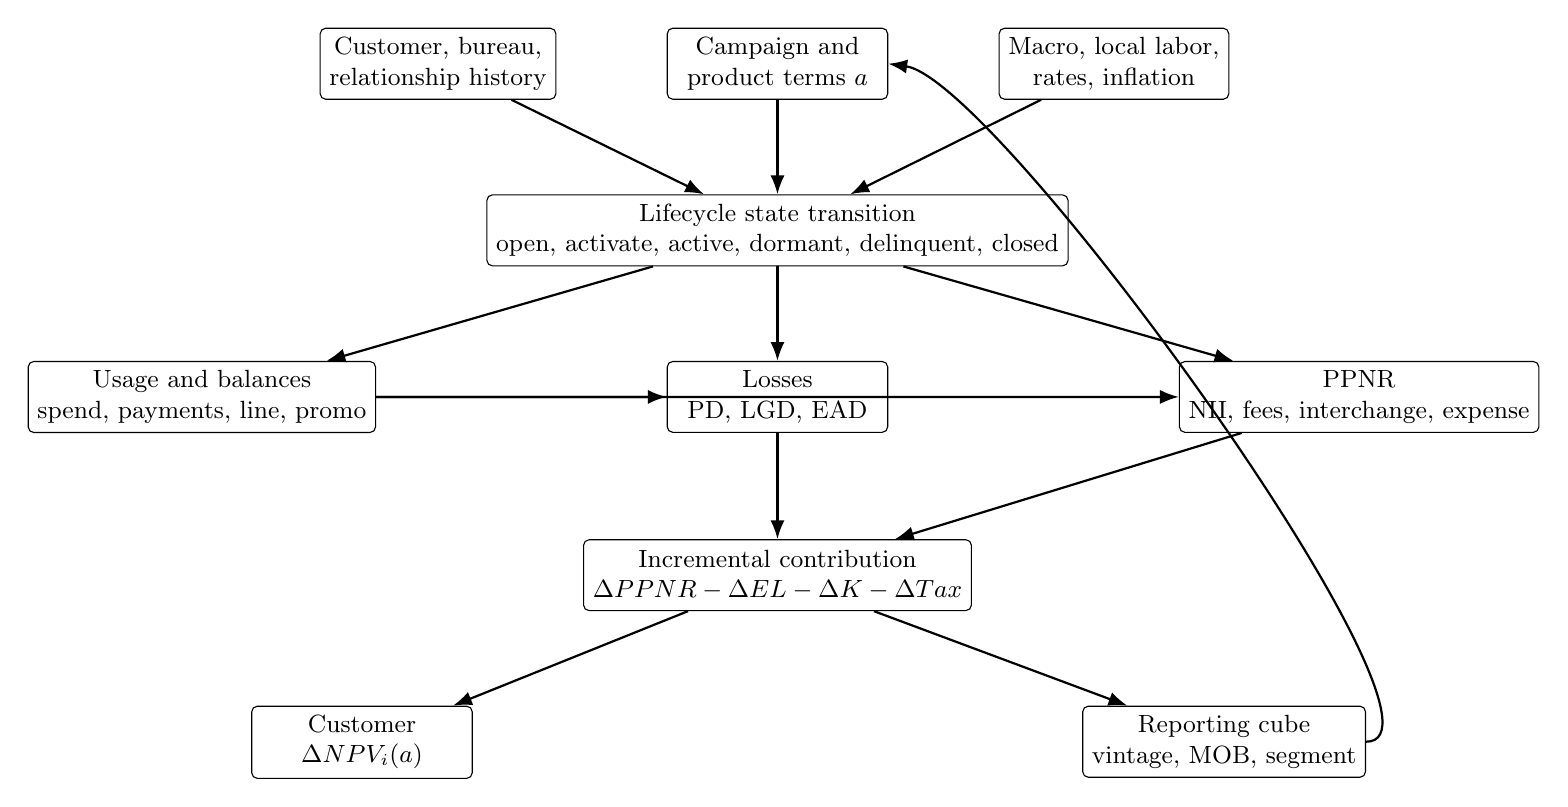
\begin{tikzpicture}[
  node distance=1.2cm and 1.4cm,
  box/.style={
    rectangle,
    draw,
    rounded corners=2pt,
    align=center,
    minimum width=2.8cm,
    minimum height=0.9cm,
    font=\small
  },
  widebox/.style={
    rectangle,
    draw,
    rounded corners=2pt,
    align=center,
    minimum width=4.0cm,
    minimum height=0.9cm,
    font=\small
  },
  arr/.style={-{Latex[length=2.4mm]}, thick}
]
\node[box] (inputs) {Customer, bureau,\\relationship history};
\node[box, right=of inputs] (offer) {Campaign and\\product terms $a$};
\node[box, right=of offer] (macro) {Macro, local labor,\\rates, inflation};

\node[widebox, below=of offer] (state) {Lifecycle state transition\\open, activate, active, dormant, delinquent, closed};

\node[box, below left=of state] (usage) {Usage and balances\\spend, payments, line, promo};
\node[box, below=of state] (loss) {Losses\\PD, LGD, EAD};
\node[box, below right=of state] (ppnr) {PPNR\\NII, fees, interchange, expense};

\node[widebox, below=1.35cm of loss] (finance) {Incremental contribution\\$\Delta PPNR-\Delta EL-\Delta K-\Delta Tax$};
\node[box, below left=of finance] (npv) {Customer\\$\Delta NPV_i(a)$};
\node[box, below right=of finance] (report) {Reporting cube\\vintage, MOB, segment};

\draw[arr] (inputs) -- (state);
\draw[arr] (offer) -- (state);
\draw[arr] (macro) -- (state);
\draw[arr] (state) -- (usage);
\draw[arr] (state) -- (loss);
\draw[arr] (state) -- (ppnr);
\draw[arr] (usage) -- (loss);
\draw[arr] (usage) -- (ppnr);
\draw[arr] (loss) -- (finance);
\draw[arr] (ppnr) -- (finance);
\draw[arr] (finance) -- (npv);
\draw[arr] (finance) -- (report);
\draw[arr] (report.east) .. controls +(1.4,0.0) and +(1.4,-0.2) .. (offer.east);
\end{tikzpicture}%
}
\caption{Schematic architecture for a component-based incremental NPV engine.}
\label{fig:component-system}
\end{figure}

\subsection{Connection Back to Incremental NPV}
\label{subsec:component-to-npv}

The component architecture is useful only if every module returns a
counterfactual cash-flow contrast. The final object should be
\begin{align}
  \Delta \NPV_i(a)
  &=
  -\Delta A_i(a)
  +
  \sum_{h=0}^{H}
  \delta_h\,
  \E\!\left[
  \begin{aligned}
    &\Delta PPNR_{i,t+h}(a)
    - \Delta EL_{i,t+h}(a)
    - \Delta K_{i,t+h}(a)\\
    &\quad
    - \Delta Tax_{i,t+h}(a)
    + \Delta RelValue_{i,t+h}(a)
    \mid \mathcal{I}_{it}
  \end{aligned}
  \right],
  \label{eq:component-delta-npv}
\end{align}
where each $\Delta$ is relative to no offer, no conversion, or the relevant
business-as-usual action. Table~\ref{tab:component-to-npv} summarizes the
handoff from each component to Equation~\eqref{eq:component-delta-npv}.

\begin{table}[t]
\centering
\caption{Component outputs required by the incremental NPV model.}
\label{tab:component-to-npv}
\begin{tabular}{p{0.20\linewidth}p{0.32\linewidth}p{0.38\linewidth}}
\toprule
Component & Required output & Connection to NPV \\
\midrule
Response and activation
  & $\Delta\Pr(\mathrm{open})$, $\Delta\Pr(\mathrm{active})$,
    $\Delta\Pr(\mathrm{first\ use})$
  & Gates all future spend, balance, expense, and loss paths. \\
Usage and balances
  & Incremental purchases, cash advances, balance transfers, payments, lines,
    promo balances, and utilization
  & Drives interchange, rewards, finance charges, funding cost, EAD, and
    capital. \\
Losses
  & $\Delta PD$, $\Delta LGD$, $\Delta EAD$, and $\Delta EL$
  & Subtracted from PPNR as expected credit loss; also informs capital and
    downside-risk constraints. \\
PPNR
  & Incremental net interest income, non-interest income, and non-interest
    expense
  & Provides pre-loss contribution before expected loss, capital, tax, and
    relationship spillovers. \\
Attrition and conversion
  & Incremental dormancy, closure, retention, and product-migration paths
  & Determines cash-flow duration and whether value is new, retained, or
    cannibalized from another bank product. \\
Relationship module
  & Incremental deposit margin and other-product contribution
  & Added only when credibly caused by the card action, preferably with
    randomized or quasi-experimental evidence. \\
Reporting segmentation
  & Aggregation by product, vintage, MOB, risk, geography, promo, and balance
    type
  & Supports governance, monitoring, and cost actions; does not by itself
    define the optimization target. \\
\bottomrule
\end{tabular}
\end{table}

This framing also clarifies what should be amended in the original
classification. Losses, balances, and PPNR are essential, but the production
system should explicitly include rewards, interchange, fraud/disputes,
servicing and collections, capital and funding, taxes/accounting, relationship
spillovers, and causal cannibalization. The model should preserve the
principal/non-principal subledger and vintage/months-on-book dimensions because
they affect both economics and governance. Finally, cost-cutting decisions
should be evaluated as actions inside the same NPV system rather than as
external heuristics; an inactive account, a promotional account, or a product
conversion is valuable only to the extent that its incremental discounted
contribution is positive after losses, costs, and cannibalization.

\section{Decision and Measurement Pitfalls in Card NPV}
\label{sec:decision-pitfalls}

The consultant concerns are well founded. They are not objections to using NPV;
they are reasons the NPV system must be explicitly staged, causal, and
uncertainty-aware. The marketing and CLV literatures support a discounted
contribution objective \citep{bult1995directmail,berger1998clv,rust2004return,venkatesan2004clv},
but the card setting adds long-horizon credit, funding, capital, and account
management dynamics. The right response is not to replace NPV with response,
approval, or sales volume. It is to make clear which NPV is being estimated, for
which decision, on which population, and under which downstream policy.

\subsection{NPV Is a Long-Horizon Latent Quantity}
\label{subsec:npv-latent}

Customer NPV is unintuitive because it is not directly observed. The bank
observes partial cash flows over finite calendar time; it does not observe the
counterfactual no-offer path, the customer's full outside-wallet behavior, or
the terminal value of the relationship. A more honest notation is therefore
\begin{equation}
  \Delta \NPV_i(a;\theta,\pi)
  =
  \sum_{h=0}^{H}
  \delta_h
  \E_\theta[
    \Delta CF_{i,t+h}(a,\pi)
    \mid \mathcal{I}_{it}
  ]
  +
  \delta_H
  \E_\theta[
    \Delta TV_{i,t+H}(a,\pi)
    \mid \mathcal{I}_{it}
  ],
  \label{eq:npv-theta-policy}
\end{equation}
where $\theta$ collects model parameters and scenario assumptions, $\pi$ is the
future account-management policy, $CF$ is the component cash flow from
Equation~\eqref{eq:component-delta-npv}, and $TV$ is terminal value. This
notation makes the instability visible: rankings can change when assumptions
about spend decay, revolve rate, attrition, default timing, recovery, funding
cost, capital cost, or terminal value change.

A bank implementation should therefore report not only
$\widehat{\Delta \NPV}_i(a)$, but also a sensitivity or posterior distribution:
\begin{equation}
  \left\{
    \Delta \NPV_i(a;\theta^{(s)},\pi^{(s)})
  \right\}_{s=1}^{S}.
  \label{eq:npv-sensitivity-draws}
\end{equation}
For campaign selection, the robust decision statistic may be expected
incremental NPV, lower-tail NPV, probability of negative NPV, or expected NPV
subject to capital and loss constraints. This is consistent with the stress-test
view that balance, revenue, and loss paths should be evaluated under macro
scenarios \citep{federalreserve2025stressmethodology,federalreserve2026stressmethodology}.
It also prevents proxy metrics such as first-90-day spend from silently becoming
promotion criteria for lifetime value.

\subsection{Card Value Is Behaviorally Heterogeneous}
\label{subsec:behavioral-heterogeneity}

The second issue is that card profitability is not one-dimensional. Two
customers with the same first-month spend can have opposite economics if one is
a low-risk transactor with high interchange and modest rewards cost, while the
other revolves promotional balances, pays slowly, uses cash advances, and later
charges off. The appropriate object is a heterogeneous treatment effect over
the full cash-flow vector:
\begin{equation}
  \tau_{V}(x,a)
  =
  \E[V_i(a)-V_i(0)\mid X_i=x],
  \label{eq:value-cate}
\end{equation}
where $V_i$ is not one outcome but the discounted contribution generated by
spend, balances, payments, losses, rewards, fraud, servicing, funding, and
capital. Uplift and causal-forest methods are useful for estimating
heterogeneous treatment effects \citep{lo2002true,wager2018causalforests,chernozhukov2018dml},
and statistical treatment-rule work emphasizes choosing actions by expected
welfare or payoff under heterogeneity rather than by average effect alone
\citep{manski2004treatment}.

This implies that the model should not rank customers by a single revenue or
risk proxy. A useful diagnostic decomposition is
\begin{align}
  \tau_{V}(x,a)
  &=
  \tau_{\mathrm{interchange}}(x,a)
  + \tau_{\mathrm{finance}}(x,a)
  + \tau_{\mathrm{fees}}(x,a)
  - \tau_{\mathrm{rewards}}(x,a) \nonumber\\
  &\quad
  - \tau_{\mathrm{servicing}}(x,a)
  - \tau_{\mathrm{fraud}}(x,a)
  - \tau_{\mathrm{loss}}(x,a)
  - \tau_{\mathrm{funding/capital}}(x,a).
  \label{eq:value-cate-decomposition}
\end{align}
The decomposition need not be estimated by separate independent models; indeed,
the components are linked through balances and states. But it should be
reported, because a high average NPV segment can hide subsegments whose value
comes from fragile assumptions about revolve, funding, or losses.

\subsection{The Evaluated Population Changes Through the Funnel}
\label{subsec:funnel-population}

The population changes as the customer moves from prospect to applicant to
approved account to booked account to active user. This is a selection problem:
the covariates observed, the eligible action set, and the conditional value
distribution all change after each gate. The sample-selection literature is the
classical warning that outcome models estimated only on selected observations
need not describe the original population \citep{heckman1979selection}. In the
card funnel, the same issue appears in operational form:
\begin{align}
  \mathcal{P}_0 &= \{i:\text{marketable prospects}\},\\
  \mathcal{P}_1 &= \{i\in\mathcal{P}_0:\text{respond or apply}\},\\
  \mathcal{P}_2 &= \{i\in\mathcal{P}_1:\text{approved and line assigned}\},\\
  \mathcal{P}_3 &= \{i\in\mathcal{P}_2:\text{booked and activated}\}.
  \label{eq:funnel-populations}
\end{align}
The right estimand changes with the conditioning set. For example,
\begin{align}
  \tau^{\mathrm{target}}(x)
    &= \E[\NPV_i(\mathrm{contact})-\NPV_i(\mathrm{suppress})
        \mid i\in\mathcal{P}_0,X_i=x],\\
  \tau^{\mathrm{approve}}(x)
    &= \E[\NPV_i(\mathrm{approve})-\NPV_i(\mathrm{decline})
        \mid i\in\mathcal{P}_1,X_i=x],\\
  \tau^{\mathrm{usage}}(x)
    &= \E[\NPV_i(\mathrm{line},\mathrm{terms})-\NPV_i(\mathrm{baseline})
        \mid i\in\mathcal{P}_2,X_i=x].
  \label{eq:funnel-estimands}
\end{align}
These are not interchangeable. A targeting model can use prospect and
relationship data but not application-only variables. An underwriting model can
use application and bureau data that were unavailable at prospect selection.
An active-account management model can use payment, utilization, transaction,
service, and delinquency history that do not exist for non-booked prospects.
Therefore, a bank should maintain separate model cards, validation populations,
and data-availability timestamps for each funnel stage.

\subsection{The Counterfactual and Objective Change by Decision}
\label{subsec:decision-counterfactuals}

The fourth issue is that ``the NPV objective'' is not one universal treatment
contrast. It is a family of decision-specific contrasts. Direct-marketing
selection asks whether contact has positive incremental value net of contact
cost \citep{bult1995directmail}. Portfolio budget allocation asks whether card
marketing beats redeploying the same budget to another product, channel, or
retention program. Underwriting asks whether approval creates value relative to
decline, subject to credit policy, fairness, compliance, and risk appetite.
Line assignment asks which line maximizes value over a feasible menu while
respecting loss and capital constraints. Formally,
\begin{equation}
  a_d^*(x)
  \in
  \arg\max_{a\in\mathcal{A}_d(x)}
  \E[
    U_d\{\Delta \NPV_i(a),Risk_i(a),Cap_i(a),Fair_i(a)\}
    \mid X_i=x,\mathcal{P}_d
  ],
  \label{eq:decision-specific-policy}
\end{equation}
where $d$ indexes the decision stage and $\mathcal{A}_d(x)$ is the feasible
action set at that stage. The utility $U_d$ may be expected NPV for low-risk
targeting, constrained NPV for underwriting, or portfolio NPV subject to budget,
capacity, capital, and fairness constraints.

Table~\ref{tab:decision-estimands} gives the operational version. The main
governance point is that a model validated for one row should not be reused for
another row without re-estimating the counterfactual and checking that the
conditioning population and action set match.

\begin{table}[t]
\centering
\caption{Decision-specific counterfactuals for card NPV.}
\label{tab:decision-estimands}
\begin{tabular}{p{0.17\linewidth}p{0.24\linewidth}p{0.24\linewidth}p{0.21\linewidth}}
\toprule
Decision & Population & Counterfactual & Objective \\
\midrule
Targeting
  & Marketable prospects or existing clients
  & Contact versus suppress
  & Incremental NPV net of campaign cost. \\
Budget allocation
  & Eligible campaign universe
  & Card campaign versus redeploy budget
  & Portfolio NPV per scarce marketing dollar or capacity unit. \\
Underwriting
  & Applicants or responders with application data
  & Approve versus decline, or approve with terms versus decline
  & Risk-adjusted NPV subject to policy and compliance constraints. \\
Line assignment
  & Approved or preapproved accounts
  & Line amount $\ell$ versus alternative line amounts
  & NPV over line menu, accounting for usage, EAD, losses, and capital. \\
Account management
  & Booked accounts
  & Maintain, reprice, retain, convert, line change, or close
  & Forward NPV under updated behavior and risk state. \\
\bottomrule
\end{tabular}
\end{table}

\subsection{Decisions Are Interdependent Over Time}
\label{subsec:interdependent-decisions}

Finally, decisions are interdependent. Acquisition changes the population that
underwriting sees. Underwriting and line assignment change the balance,
utilization, and risk states that account management later sees. Future line,
pricing, collections, retention, or conversion policies change the lifetime
economics assumed at acquisition. The dynamic treatment-regime and Markov
decision-process literatures provide the natural language for this problem:
the value of an action depends on the future policy that follows it
\citep{puterman1994mdp,murphy2003dynamic,rust1987replacement}.

A compact representation is
\begin{align}
  Z_{i,t+1} &\sim p_\theta(Z_{i,t+1}\mid Z_{it},X_{it},a_t),\\
  CF_{it}  &= c_\theta(Z_{it},X_{it},a_t),\\
  \pi_t    &: (Z_{it},X_{it}) \mapsto a_t,
  \label{eq:dynamic-policy-system}
\end{align}
with policy value
\begin{equation}
  V^\pi_i(z,x)
  =
  \E_\theta^\pi
  \left[
    \sum_{h=0}^{H}\delta_h CF_{i,t+h}
    + \delta_H TV_{i,t+H}
    \mid Z_{it}=z,X_{it}=x
  \right].
  \label{eq:policy-value}
\end{equation}
The acquisition model should therefore state its assumed downstream policy
$\pi$: for example, line-increase rules, repricing rules, collections policy,
retention offers, dormancy closure, and product-conversion policy. If those
policies change, the upstream acquisition NPV should be recalibrated. This is
especially important for cost-cutting initiatives: closing inactive accounts,
reducing promotional offers, tightening lines, or converting products may
improve near-term expense or losses while reducing the value of cohorts that
were acquired under older assumptions.

The practical recommendation is to treat card NPV as a policy-evaluation
system, not a one-time score. Each major decision should store the population,
available variables, action set, counterfactual, downstream policy assumption,
cash-flow decomposition, and sensitivity range. That metadata is not bureaucracy;
it is what prevents an upstream model from optimizing a downstream world that
the bank no longer operates.

\section{Empirical Design and Validation}
\label{sec:validation}

\subsection{Data requirements}

A bank-grade data set should join campaign exposure, channel, creative, offer
terms, application, underwriting, activation, card transactions, balances,
payments, delinquency, charge-off, recoveries, fraud, disputes, servicing,
relationship products, deposits, payroll indicators, bureau refreshes, and
local macro series. The data should preserve timing. Variables measured after
campaign exposure must not be used as if they were available at targeting time.

For the existing-client new-card problem, the data must also identify
cannibalization. At minimum, the bank should measure whether new-card spend
comes from:
\begin{enumerate}[label=\alph*.]
  \item genuinely incremental customer spend;
  \item spend shifted from a competitor card;
  \item spend shifted from the bank's existing card;
  \item debit or deposit activity shifted onto credit;
  \item temporary promotion-induced spend that decays after the offer.
\end{enumerate}
Only the first two categories are necessarily positive for the issuing bank, and
even those must be netted against rewards, losses, and costs.

\subsection{Promotion criteria}

The primary promotion criterion should be randomized or credibly
quasi-experimental lift in incremental NPV. Response AUC, approval AUC,
activation lift, first-purchase lift, and first-90-day spend are useful
diagnostics, but they are proxy metrics. They should nominate models for
further testing rather than establish lifetime NPV validity.

Recommended validation splits include:
\begin{itemize}[leftmargin=*]
  \item time-based holdouts for economic drift;
  \item campaign randomized holdouts for treatment effects;
  \item vintage holdouts for lifetime trajectories;
  \item macro-stress backtests around unemployment, rate, and inflation shocks;
  \item segment calibration across score bands, income proxies, geography,
        tenure, relationship depth, channel, and product;
  \item counterfactual cannibalization analysis for existing-client offers.
\end{itemize}

\section{Open Gaps and Reviewer Risks}

The public literature does not fully identify issuer-specific new-card usage
and incremental NPV. Payment-choice and rewards studies show mechanisms, but
the activation probability for a particular bank, product, offer, channel, and
customer segment is a proprietary empirical object. Likewise, CLV models provide
powerful baselines for transaction frequency and duration, but bank NPV requires
integration with expected credit loss, rewards, fraud, funding, capital, and
regulatory constraints.

The largest reviewer risks are:
\begin{enumerate}[label=\arabic*.]
  \item treating activation or first spend as lifetime NPV evidence;
  \item treating raw propensity as causal lift;
  \item ignoring cannibalization from the bank's existing cards;
  \item estimating spend without macro and employment state dependence;
  \item separating marketing CLV from credit risk and balance-sheet cost;
  \item using public rewards estimates as universal program parameters;
  \item reusing one NPV model across targeting, underwriting, line assignment,
        and account management without changing the counterfactual;
  \item validating on booked or active accounts while applying the result to
        prospects or applicants without correcting for funnel selection.
\end{enumerate}

\section{Source-Support Audit}
\label{sec:audit}

This paper is a structured literature survey for product and model-design
purposes. It is not yet a complete model-governance literature audit. Primary
source pages, abstracts, and working-paper summaries were inspected on
June~26--27, 2026. Full-text technical sections, appendices, citation-count
metadata, retraction checks, and full backward/forward snowballing remain open.
Table~\ref{tab:source-support} records how the main sources are used.

\begin{longtable}{p{0.23\linewidth}p{0.20\linewidth}p{0.47\linewidth}}
\caption{First-pass source-support ledger.}
\label{tab:source-support}\\
\toprule
Source & Classification & Use in this paper \\
\midrule
\endfirsthead
\toprule
Source & Classification & Use in this paper \\
\midrule
\endhead
\citet{bult1995directmail}
  & Direct marketing optimization
  & Supports the claim that campaign selection is normally an expected-profit
    problem, not a response-probability problem alone. \\
\citet{berger1998clv}, \citet{rust2004return}, and \citet{venkatesan2004clv}
  & CLV and customer-equity foundations
  & Support the discounted-contribution framing; the paper's credit-card NPV
    equation is a bank-specific extension with loss, capital, funding, fraud,
    rewards, and cannibalization terms. \\
\citet{ganong2019unemployment}
  & Household finance
  & Supports the claim that labor-income and unemployment events affect
    high-frequency spending and should enter spend forecasts. \\
\citet{johnson2004rebates}
  & Income-shock evidence
  & Supports the claim that liquidity and transfer timing can produce
    heterogeneous short-run spending responses. \\
\citet{gross2001liquidity}
  & Credit-card account evidence
  & Supports the claim that credit limits and interest rates affect card debt
    behavior and interact with liquidity constraints. \\
\citet{agarwal2013cardact}
  & Credit-card regulation evidence
  & Supports the claim that fees, disclosures, and payment nudges are material
    NPV components and governed levers. \\
\citet{baker2020epidemic}
  & Macro-shock evidence
  & Supports the claim that major shocks can alter spending levels and
    category composition. \\
\citet{koulayev2012payment}
  & Payment-choice model
  & Supports the distinction between payment-instrument adoption and use. \\
\citet{agarwal2010rewards}
  & Rewards and usage evidence
  & Supports the claim that rewards can shift card spend and debt; not used as a
    universal activation-rate estimate. \\
\citet{prelec2001creditcard}
  & Behavioral mechanism
  & Supports the mechanism that payment method can affect purchase behavior;
    not used for portfolio calibration. \\
\citet{schmittlein1987counting}, \citet{fader2005bgnbd}, and \citet{fader2005rfm}
  & CLV foundations
  & Support use of transaction-frequency, recency, monetary-value, and active
    status models as components of card lifetime modeling. \\
\citet{bolton1998duration}
  & Duration model
  & Supports use of relationship-duration or hazard components for attrition
    and dormancy. \\
\citet{bcbs2006basel}
  & Regulatory capital framework
  & Supports PD/LGD/EAD terminology and the use of exposure, default
    probability, and severity as separate risk components; not a marketing NPV
    optimization paper. \\
\citet{fasb2016asu201613}
  & Accounting standard
  & Supports lifetime expected-credit-loss framing under current conditions
    and reasonable forecasts; not used to define customer-level causal lift. \\
\citet{federalreserve2025stressmethodology} and
\citet{federalreserve2026stressmethodology}
  & Supervisory stress-test methodology
  & Support bank-level separation of projected losses, balances, revenues, and
    PPNR under macro scenarios; used here as architecture support, not as a
    customer-acquisition estimator. \\
\citet{hand1997credit}, \citet{thomas2000survey}, and
\citet{lessmann2015benchmarking}
  & Credit-scoring surveys and benchmark
  & Support use of application and behavioral scoring methods for PD and
    delinquency/default components; not used to choose one production model. \\
\citet{schuermann2004lgd}
  & LGD survey
  & Supports modeling LGD as a severity/recovery object distinct from PD and
    EAD, with macro and workout-state dependence. \\
\citet{rosenbaum1983propensity}, \citet{lo2002true},
\citet{wager2018causalforests}, and \citet{chernozhukov2018dml}
  & Causal/uplift methods
  & Support methodological framing for treatment effects; not bank-specific
    evidence. \\
\citet{heckman1979selection}
  & Sample-selection foundation
  & Supports the warning that models estimated after response, approval, or
    booking need not describe the original prospect population. \\
\citet{manski2004treatment}
  & Statistical treatment rules
  & Supports choosing actions by expected payoff under heterogeneous effects,
    rather than ranking by a single average response or risk measure. \\
\citet{puterman1994mdp}, \citet{murphy2003dynamic}, and
\citet{rust1987replacement}
  & Dynamic decision and policy-value methods
  & Support representing acquisition, underwriting, line assignment, and account
    management as linked sequential decisions whose value depends on downstream
    policy. \\
\bottomrule
\end{longtable}

No paper in this survey is used to conclude a universal activation rate, spend
elasticity, or NPV parameter. The activation and cannibalization parameters for
a large U.S. retail bank should be estimated from internal experiments or
credible quasi-experiments.

\section{Conclusion}

Estimating the NPV of a new credit card customer requires a joint model of
marketing response, payment-instrument use, lifetime spend, revolving balances,
risk, cost, and macro state dependence. The literature provides strong evidence
for several components: income and employment affect spending, liquidity and
credit terms affect card debt, adoption differs from use, rewards can change
usage, and CLV models can forecast transaction and duration components. It does
not provide a universal public formula for whether an existing bank client will
use a particular new card or what that customer's incremental NPV will be. That
object is bank-, product-, campaign-, and state-specific. A defensible bank
model should therefore combine public-literature mechanisms with internal
randomized or quasi-experimental lift measurement and should promote models on
incremental risk-adjusted NPV rather than raw response or spend propensity.

\bibliographystyle{plainnat}
\bibliography{credit_card_npv_refs}

\end{document}
